\documentclass[10pt,a4paper]{report}
\usepackage[latin1]{inputenc}
\usepackage{amsmath}
\usepackage{amsfonts}
\usepackage{amssymb}
\usepackage{graphicx}
\usepackage{tikz}
\usetikzlibrary{arrows,shadows,positioning}
\begin{document}
	\title{A Framework for Developing Distributed Protocols with Event-B/Rodin: \vspace{.5cm} \\ \large Graphical Language Notes}
	\author{Paulius Stankaitis and Alexei Iliasov}
	\date{}
	\maketitle
	\section*{Leader Election Protocol (Synchronous Ring)}
	In the first example we use (modified) Le Lann, Chang and Roberts (LCR) algorithm to solve leader election problem. The algorithm uses only unidirectional communication and does not rely on knowledge of the size of the ring. Only the leader performs an output. The algorithm uses only comparison operations on the unique identifiers [A. Lynch: Distributed Algorithms, p. 27]. \\
	

		\begin{itemize}
			\item All processes send identifier around the ring.
			\item Upon receiving an incoming identifier, it compares to its own.
			\item If identifier is greater than its own, keep passing the identifier.
			\item If received identifier is smaller, discard identifier.
			\item If identifier is equal to its own, declare itself the leader.
			\item Leader sends a report message around the ring.
			\item Upon receiving a report message process halts.
		\end{itemize}
		
	\begin{center}
		

		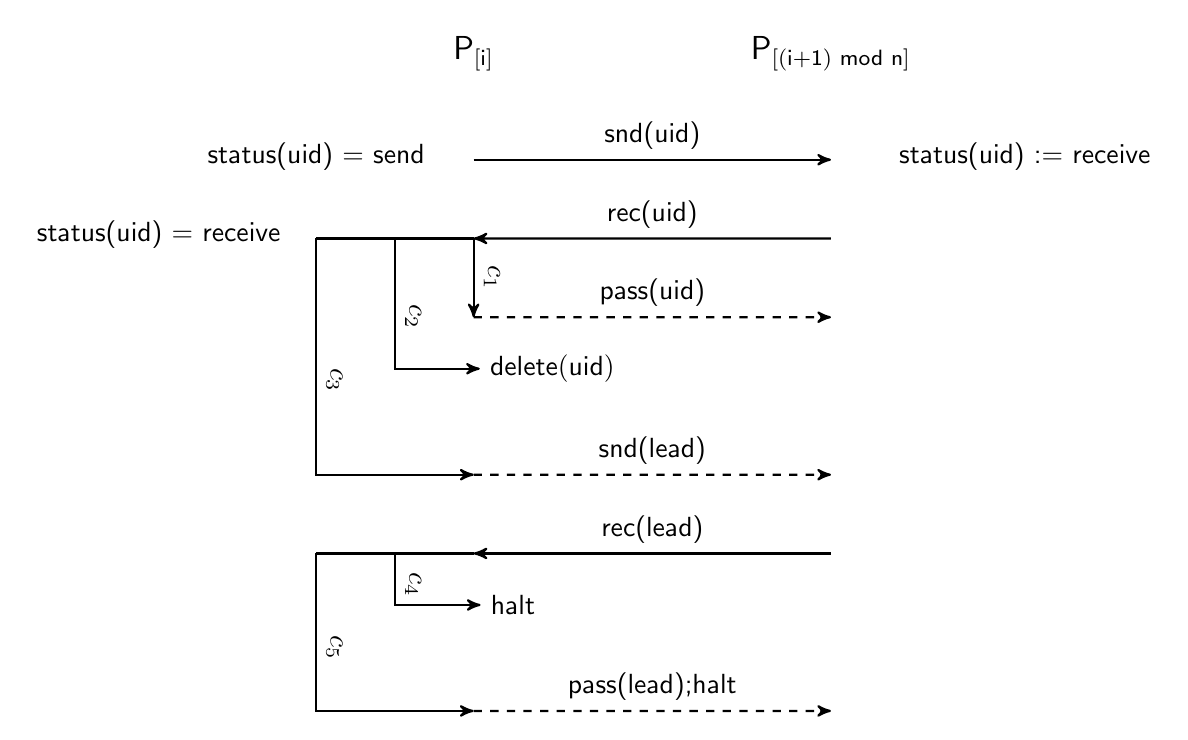
\begin{tikzpicture}[font=\sffamily,>=stealth',thick,
		commentl/.style={text width=3cm, align=right},
		commentr/.style={commentl, align=left},]
		\node[] (init) {\large $\mathsf{P_{[i]}}$};
		\node[right=3cm of init] (recv) {\large $\mathsf{P_{[(i+1) \hspace{.1cm} mod \hspace{.1cm} n]}}$};
		
		\draw[->] ([yshift=-1cm]init.south) coordinate (fin1o) -- ([yshift=0cm]fin1o-|recv) coordinate (fin1e) node[pos=.5, above, sloped] {snd(uid)};
		
	\node at (-2, -1.3) {status(uid) = send};

	\node at (7, -1.3) {status(uid) := receive};
	
	\node at (-4, -2.3) {status(uid) = receive};
	
	
		\draw[->] ([yshift=-1cm]fin1o-|recv) coordinate (fin2e) -- ([yshift=-2cm]init.south) coordinate (fin2o) node[pos=.5, above, sloped] {rec(uid)};
		
		
		
				
		\draw[->, dashed] ([yshift=-3cm]init.south) coordinate (fin3o) -- ([yshift=-2cm]fin1o-|recv) coordinate (fin3e) node[pos=.5, above, sloped] {pass(uid)};
		
		\node at (1, -4) (fin4o) {\normalsize $\mathsf{delete(uid)}$};
		
			\draw  (fin2o) --  ([yshift=-2cm, xshift=-1cm]init.south) coordinate (t2) ; 
			\draw[->] (t2) |-  (fin4o) node[pos=.3, above, sloped] {\normalsize $c_2$}; 
	
		\draw[->]  (fin2o) --  (fin3o) node[pos=.5, above, sloped] {\normalsize $c_1$}; 
		
		\draw[->, dashed] ([yshift=-5cm]init.south) coordinate (fin5o) -- ([yshift=-4cm]fin1o-|recv) coordinate (fin5e) node[pos=.5, above, sloped] {snd(lead)};
		
		\draw  (fin2o) --  ([yshift=-2cm, xshift=-2cm]init.south) coordinate (t1) ; 
		\draw[->] (t1) |-  (fin5o) node[pos=.3, above, sloped] {\normalsize $c_3$}; ; 
		
		\draw[->] ([yshift=-5cm]fin1o-|recv) coordinate (fin6e) -- ([yshift=-6cm]init.south) coordinate (fin6o) node[pos=.5, above, sloped] {rec(lead)};
		

				
		\draw[->, dashed] ([yshift=-8cm]init.south) coordinate (fin8o) -- ([yshift=-7cm]fin1o-|recv) coordinate (fin8e) node[pos=.5, above, sloped] {pass(lead);halt};
	
	\draw  (fin6o) --  ([yshift=-6cm, xshift=-2cm]init.south) coordinate (t2) ; 	
	\draw[->] (t2) |- (fin8o) node[pos=.3, above, sloped] {\normalsize $c_5$};
	
	\node at (.5, -7) (fin9o) {\normalsize $\mathsf{halt}$};
	
		\draw  (fin6o) --  ([yshift=-6cm, xshift=-1cm]init.south) coordinate (t3) ; 
		\draw[->] (t3) |-  (fin9o) node[pos=.3, above, sloped] {\normalsize $c_4$}; 
		
		\end{tikzpicture}
	\end{center}
	
		\noindent\fbox{%
			\parbox{\textwidth}{%
				$\mathsf{Everyone \hspace{.1cm} Eventually \hspace{.1cm} Halts; Leader \hspace{.1cm} Elected}$
			}%
		} \\
	
	$\mathsf{\hspace{.5cm} c_1 = [rec(uid) > snd(uid)]} \hspace{.5cm} \mathsf{c_2 = [rec(uid) < snd(uid)]} \hspace{.5cm}\vspace{.2cm} \mathsf{c_3 = [rec(uid) = snd(uid)]}\hspace{.5cm} \\  \mathsf{c_4 = [f_{uid}(lead) = f_{p}(uid)]} \hspace{.5cm} \mathsf{c_5 = [f_{uid}(lead) \neq f_{p}(uid)]}$ \\
	

	
	\pagebreak
	\noindent \textbf{Comments:}
	
	\begin{itemize}
		\item $P_{[i]}$ always sends a message to $\mathsf{P_{[(i+1) \hspace{.1cm} mod \hspace{.1cm} n]}}$ where n is the number of processes.
		\item In contrary to other protocols (e.g. distr. resource allocation) the source of received message is irrelevant (same destination) for this protocol.
	
			\item Message types patterns $\mathsf{[when, where, status] \hspace*{.1cm} message}$;
	
			\item Initiating messages such as $\mathsf{snd(uid)}$ typically don't have $\mathsf{when}$ part.
			\item A reply message has $\mathsf{when}$ guard part.
			\item Status variable for reasoning about protocols.
			\item $\mathsf{status(p_1) := start \rightarrow \cdot \rightarrow status(p_1) := consensus}$
			\item $\mathsf{status(p_1) := state_1 \rightarrow Guards \rightarrow status(p_1) := state_2}$
			\item Use flow plug-in to verify process state transition.
				\item Capturing processes knowledge;
				\begin{itemize}
					\item message content;
					\item topology;
				\end{itemize}

	\end{itemize}
	
	\newpage
	\section*{Dinning Philosophers Protocol}
	
	\newpage
	\section*{Distributed Resource Allocation Protocol}
\end{document}